\documentclass[letter]{ieice}
\usepackage[ruled,linesnumbered]{algorithm2e}
\usepackage{amssymb,amsthm,amsmath}
\usepackage{balance}
\usepackage{graphicx}          % graphicx package for including ps files  
\usepackage{epsfig}
\usepackage{url}
\usepackage{subfigure}
\usepackage{algorithmic}
\usepackage{float}
\newtheorem{theorem}{Theorem}[section]
\newtheorem{lemma}[theorem]{Lemma}
\usepackage{latexsym}
\usepackage{multirow}
\usepackage{color}
\usepackage{url}
\usepackage{comment}
%\usepackage{pstricks}
\usepackage{epstopdf}

\setcounter{page}{1}
%\breakauthorline{}% breaks lines after the n-th author

\field{D}
%\SpecialIssue{}
%\SpecialSection{}
%\theme{}
\title{SEDONA: A Novel Protocol for Identifying Infrequent, Long-Running Daemons on a Linux System}
%\titlenote{This work was in part supported by the EDISON program (NRF-2011-0020576).}
%\titlenote{}
\authorlist{
 \authorentry[yksuh@kisti.re.kr]{Young-Kyoon SUH}{m}{labelA}
 %\authorentry[rts@cs.arizona.edu]{Richard T. Snodgrass}{n}{labelB}}
\affiliate[labelA]{Supercomputing R\&{D} Center, KISTI, 245 Daehangno, Yuseong-gu, Daejeon, 34141, Republic of Korea}
%\affiliate[labelB]{Department of Computer Science, University of Arizona, Tucson, AZ 85721, USA}
}
\received{2016}{11}{30}
%\revised{2015}{10}{31}

\definecolor{grey}{RGB}{200,200,200}
\newcommand{\hilite}[1]{\colorbox{grey}{#1}}
\newcommand{\hilitey}[1]{\colorbox{yellow}{#1}}
\newcommand{\hiliting}[1]{\colorbox{grey}{#1}}
\long\def\todo#1{\hilitey{{\bf TODO:} {\em #1}}}
\long\def\shorten#1{}
\long\def\comment#1{}

\begin{document}

\maketitle

\begin{summary}
It is challenging to accurately measure the execution-time of a given
program due to many extraneous factors. To enable better timing results
restrained, we present a novel protocol that identifies infrequent,
long-running daemons to enable effective elimination of executions
exhibiting these daemons.

\end{summary}
\begin{keywords}
Infrequent Long-running Daemon, Execution-Time Measurement
\end{keywords}

\section{Introduction}
\label{sec:intro}

Measuring program execution time is a much-used
technique for performance evaluation in computer science. 
Despite the importance of accurate and precise execution-time measurement, 
how to achieve {\em better} timing has not been well addressed. 
Surprisingly, there is considerable variability in the measured time, 
which indeed suggests the need for a better timing protocol.

Consider a simple compute-bound program, termed {\em PUT} (program-under-test), 
as shown in Fig.~\ref{alg:put}. 
This program runs a nested for-loop with a specified task length ($tl$) (in seconds). 
The $tl$ value is translated to the corresponding 
number of iterations for which that for-loop is performed. 

\vspace{-.25in}
\begin{figure}[h]
\begin{center}
\begin{algorithmic}
{\bf Algorithm} PerformManyIncrements($tl$): \\
\STATE $t$ = TranslateToNumRepeats($tl$) \\
\FOR{$k$ = 1 to $t$ by 1}
	\FOR{$i$ = 1 to {UINT\_MAX}-1 by 1}
		\STATE $j$ += 1 \\
	\ENDFOR 
\ENDFOR 
\end{algorithmic}
\end{center}
\caption{Task Definition by a Program-Under-Test (PUT)\label{alg:put}}
\vspace{-.25in}
\end{figure}

\begin{figure}[t]
	\centering
	\subfigure[Initial Elapsed Time Measurement]{
		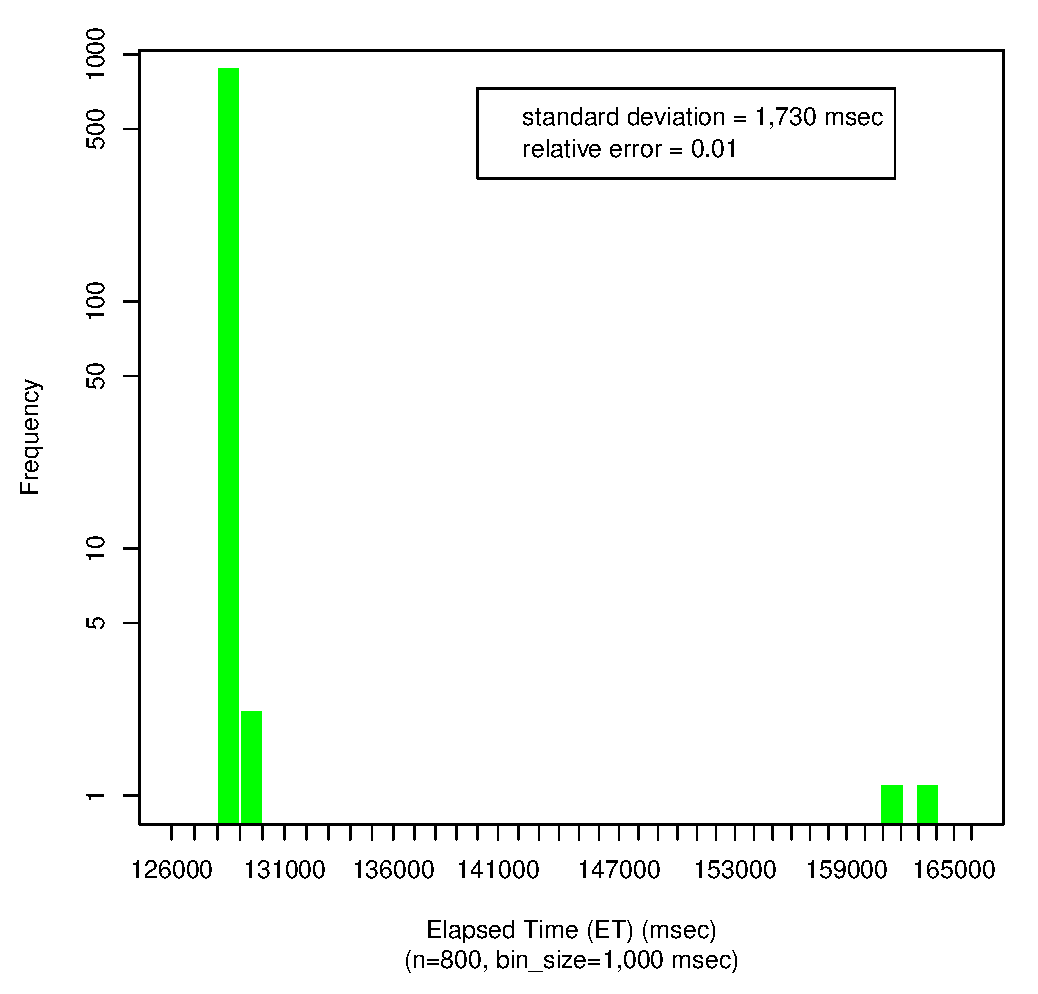
\includegraphics[width=0.32\textwidth]{128_sec_et_old_hist.eps}
		\label{fig:hist_before_et}
	}
	\subfigure[Program Time After Identified Daemon Removal]{
		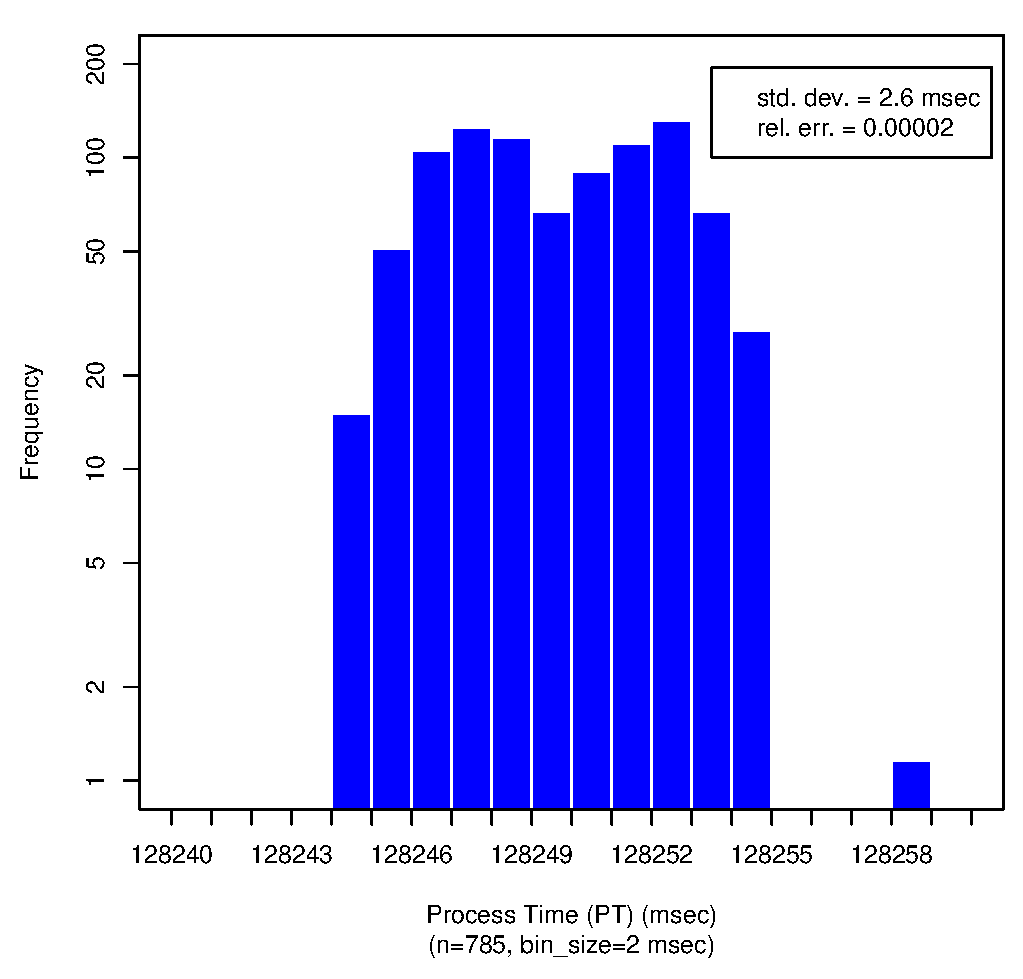
\includegraphics[width=0.32\textwidth]{128_sec_pt_new_hist.eps}
		\label{fig:hist_after_pt}
	}
	\caption{An Example of Measurement Results on a \linebreak \hbox{Compute-bound} 
	Program-Under-Test~\label{fig:meas_comp}}
	\vspace{-.3in}
\end{figure} 

We used 128~seconds as the task length ran the PUT program (designated as PUT128) 
800~times. Fig.~\ref{fig:meas_comp} shows two histograms of the timing results on the PUT128.
As can be seen in Fig.\ref{fig:hist_before_et}, 
most of the 800 executions measured in elapsed time, 
via  {\tt System.currentTimeMillis()} in Java, are gathered in the tallest bar 
of \hbox{128,000--129,000 msec,} with just a few executions outside of that bar. 
But these outliers seriously hurt the overall measurement quality: 
a standard deviation of 1,700 msec and a relative error of 0.03. 
\shorten{This result suggests adequately eliminating these outliers 
while retaining most of the measured executions.}

In contrast, our scheme, which we propose shortly, 
significantly reduces such variability.
The gist of the scheme is to (i)~focus on
{\em process time} (PT) rather than on elapsed time (ET) and 
(ii)~remove some executions that involve
{\em infrequent, \hbox{long-running} daemon processes}, which impact
the process time of the process. 
%(Typically, one tick is equivalent to 1/100 secs, or 1 {\tt HZ}.) 
Using PT is preferred, in that it considers 
the time taken for only a process of interest.
PT can be calculated as the sum of ticks (where one tick is equal to 10 msec)
in user and system mode, available via {\tt taskstats} C struct, 
provided by the Linux NetLink facility~\cite{Netlink}.
This use of PT and selective elimination 
results in improved 
measurement quality---in both standard deviation and relative error---
by three orders of magnitude, 
as illustrated in Fig.~\ref{fig:hist_after_pt}. 

{\bf Related Work.} 
McGeoch introduced
two basic methods of measuring program time: elapsed time and CPU time~\cite{Mcgeoch12}. 
Bryant and O'Hallaron~\cite{Randal03} 
presented two timing schemes of using clock-cycle and interval counters. 
They proposed a measurement protocol, called {\em minimum-of-k}, 
that for observed elapsed ticks the minimum is chosen as the most accurate one. 
Odom et al.'s work~\cite{Odom05} focuses on timing long-running programs 
in a simulation framework via 
dynamic sampling of trace snippets during program execution. 
None of these prior works, however, takes into account the variability in 
timing and the influence of daemons that may significantly disturb the timing.

%Some prior works~\cite{Burns93,Grund11,Santos10,Wilhelm08} discuss 
%the worst case execution time (WCET) of a process. 
%The papers focused on measuring the WCET of a deadline-sensitive process 
%on real-time embedded systems while being oblivious to 
%daemons coexisting with the process. In addition, we do not consider real-time constraints. 

Commercial software tools measure execution time~\cite{VTune,TimeSys,WindView}. 
Since the tools' source code is not disclosed, there is no way of figuring out 
whether they can prevent such a daemon from timing. 

We previously developed a timing protocol called TTP (Tucson Timing Protocol)
for programs exhibiting I/O, in particular, query execution time in \hbox{DBMSes}~\cite{Currim}.
Our study identified a variety of Linux measures 
(e.g., user ticks, system ticks, IOWait ticks, etc.) 
relevant to timing a single query and then 
presented a structural causal model 
of explicating the variance of query time. 
Based on this model, we proposed the protocol for calculating the query time. 
Our scheme we propose in this manuscript 
is applicable to the TTP protocol, to further improve the query time calculation.

{\bf Contribution.} 
Our contributions are following.
\vspace{-0.05in}
\begin{itemize}

\item We provide empirical evidence that 
measuring program time 
can be seriously affected by extant system daemons.

\item We propose a novel timing protocol that
identifies infrequent, long-running daemons that impact the timing results for that program. 
%This scheme determines in a disciplined way cutoffs to remove executions with such daemons.

\item We evaluate the performance of the protocol with rigorous experiments, 
starting from a simple program in pure-computation mode 
to a popular industrial benchmark suite.

%\item We examine how the FIND scheme applies to process time as well as elapsed time.

\item The experimental results show a demonstrate for the effectiveness of our scheme\shorten{SEDONA: 
early eliminating dirty executions infected with such a daemon 
and eventually contributing to enhancing the overall measurement-quality}. 

\end{itemize}
\vspace{-0.05in}

\noindent
The rest of this letter is organized as follows. 
Section~\ref{sec:prop_appach} elaborates on the proposed scheme. 
In the following section, we evaluate the performance of 
the scheme using real workloads.

%\vspace\fill

\section{Proposed Scheme}
\label{sec:prop_appach}

In this section we propose a novel execution-time measurement scheme, 
called {\em SEDONA} (Selective Elimination through Detection of infrequent, lOng-ruNning dAemons). 
Our scheme catches and eliminates executions including daemon processes that are infrequent and 
long-running via a {\em cutoff} measure, and significantly improves measurement quality. 
The SEDONA scheme consists of a total of ten steps, as described in Fig.~\ref{alg:find}. 
%We first enumerate the steps to (a)~identify infrequent, 
%long-running daemons, using a single run of many executions of PUT128, 
%(b)~refine the list using a single run of many executions of PUT16384 (with a task length of 16K sec), 
%and then (c)~use the data from those two runs to determine the cutoff for 
%each \hbox{so-identified} daemon. 
%We can then apply these cutoffs to remove outliers from subsequent runs of any 
%arbitrary PUT and realistic workloads.
%\vspace{-0.22in}

\begin{figure}[h]
\begin{center}
\begin{algorithmic}
{\bf Algorithm} The SEDONA Timing Scheme: \\
\STATE Step 1. Set up the timing environment.
\STATE Step 2. Perform a single PUT run (specifically, PUT128) for many samples (specifically, 800).
\STATE Step 3. Consider each pair of elapsed time measurements to be a
dual-PUT measurement 
and examine a scatter-plot to see if it it displays an $L$-shape.
\STATE Step 4. Zoom into the central cluster to ensure that it is symmetric (roughly circular).
\STATE Step 5. Compute the maximum and standard deviation of the process time 
for each daemon encountered within the central cluster samples.
\STATE Step 6. Identify for each sample in the $L$-shape infrequent, long-running daemon executions. 
\STATE Step 7. Determine potentially periodic daemons based on the $L$-executions 
and for each daemon compute the minimum process time from those executions identified. 
\STATE Step 8. Perform Steps 1--6 above for a single run 
consisting of a small number of executions (specifically, 40) of PUT16384.  
\STATE Step 9. Compute the cutoffs for each identified daemon. 
\STATE Step 10. Discard an execution including a daemon of which process
time is greater than the respective cutoff time.
\end{algorithmic}
\end{center}
\caption{Summary of the SEDONA Scheme\label{alg:find}}
\vspace{-0.28in}
\end{figure}
%

%We now elaborate the SEDONA scheme with an example, to explain and justify each step.
%\vspace{-0.8in}

%\subsection{A Running Example} 
%\vspace{-0.05in}
{\bf A Running Example.} 
As motivated by our prior work~\cite{Currim}, 
we configure a timing environment by i) stopping non-critical daemons, 
ii) activating the Network Timing Protocol daemon, and 
iii) switching off particular CPU features\cite{intel15,intelSpeed15} if any (Step 1). 
%(Our machine's specification will be given in Tab~\ref{tab:machine_config}).

We then run a program-under-test (called PUT) of 
Fig.~\ref{alg:put} with a task length of 128~sec, 
termed {\em PUT128}, 800 times (Step 2). 
(We render Fig.~\ref{fig:hist_before_et} using the 800 samples from this run.)
We use 128 seconds because that is long enough to perhaps experience an infrequent daemon. 
We run it 800 times to capture infrequent daemons that perhaps run every few hours or even 
once a day. 
Note that we collect all daemon processes as well as the PUT and their measures 
through the Netlink interface from the kernel before and after each 
timing.

Fig.~\ref{fig:reg_put128} plots all the 800 elapsed times of the run of PUT128.
%We see three rows in the plot: a solid row of many samples, perhaps
%six or more samples that are just above that solid row, and two
%samples that are way above the solid row. 
The plot clearly shows three rows; that is, 
the top and middle rows represent over a dozen of outliers far from 
the rest of the samples clustered in the bottom row. 
We'll now drill down into these outliers to 
show how to reliably eliminate the indirect influence of 
some ``infrequent, long-running daemons'' on the process time (PT) 
of the PUT.

To identify such daemons, we use a novel scatter plot: 
those of {\em pairs of successive samples}.\shorten{So samples 1 and 2 
form the first pair, samples 3 and 4 form the second pair.} 
Fig.~\ref{fig:raw_put128} presents such a scatter plot 
of 400 samples of a \hbox{dual-PUT256} constructed 
from a run of the 800 PUT128 samples (Step~3). 
There are two quite obvious outliers\shorten{, corresponding to sample \# 75 and \# 634,} with ETs of 163,913 msec (rightmost) and 161,785 msec (uppermost), respectively. 

\begin{figure}[t]
	\centering
	\subfigure[PUT128 with 800 Samples]{
		%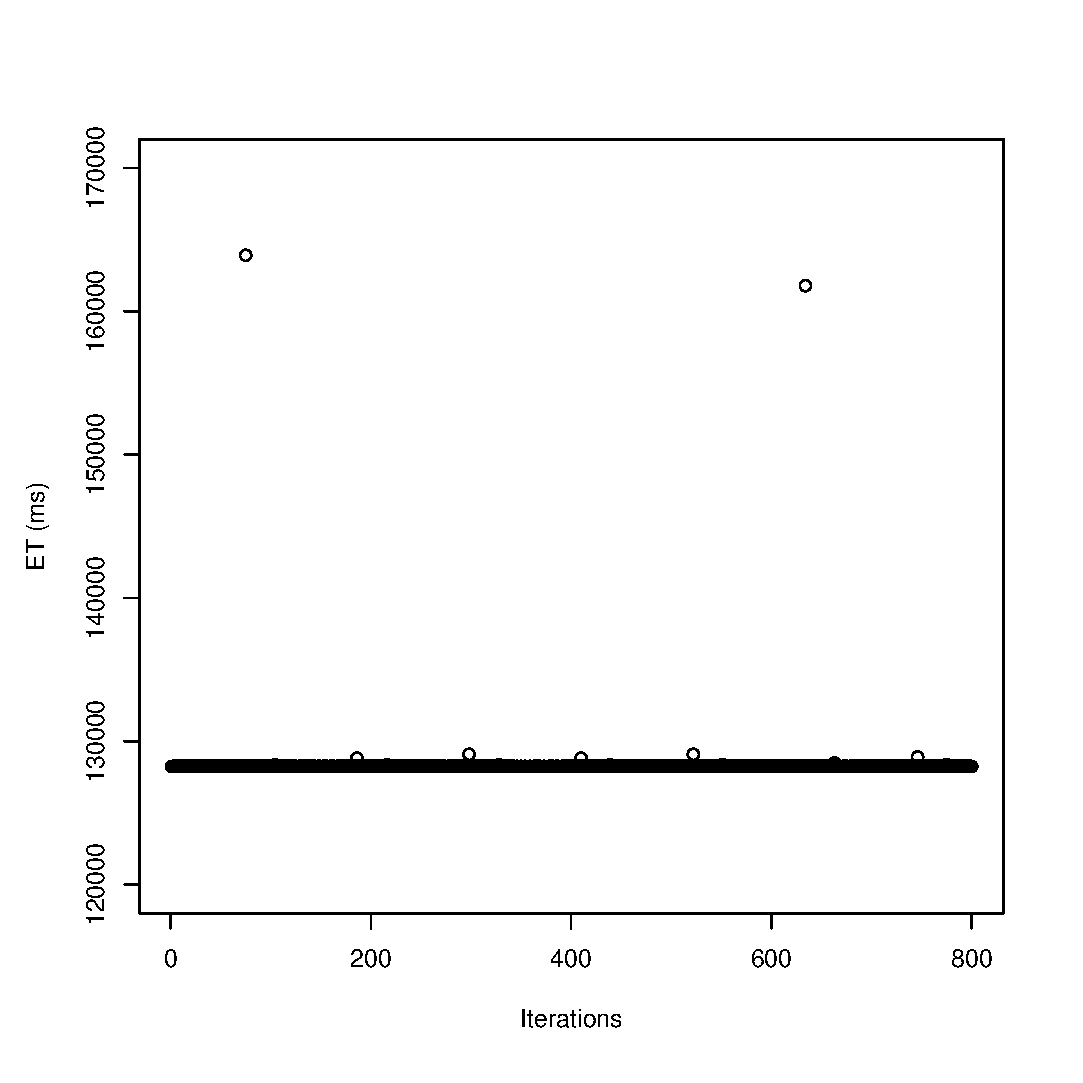
\includegraphics[width=0.223\textwidth]{put128_empv4.eps}
		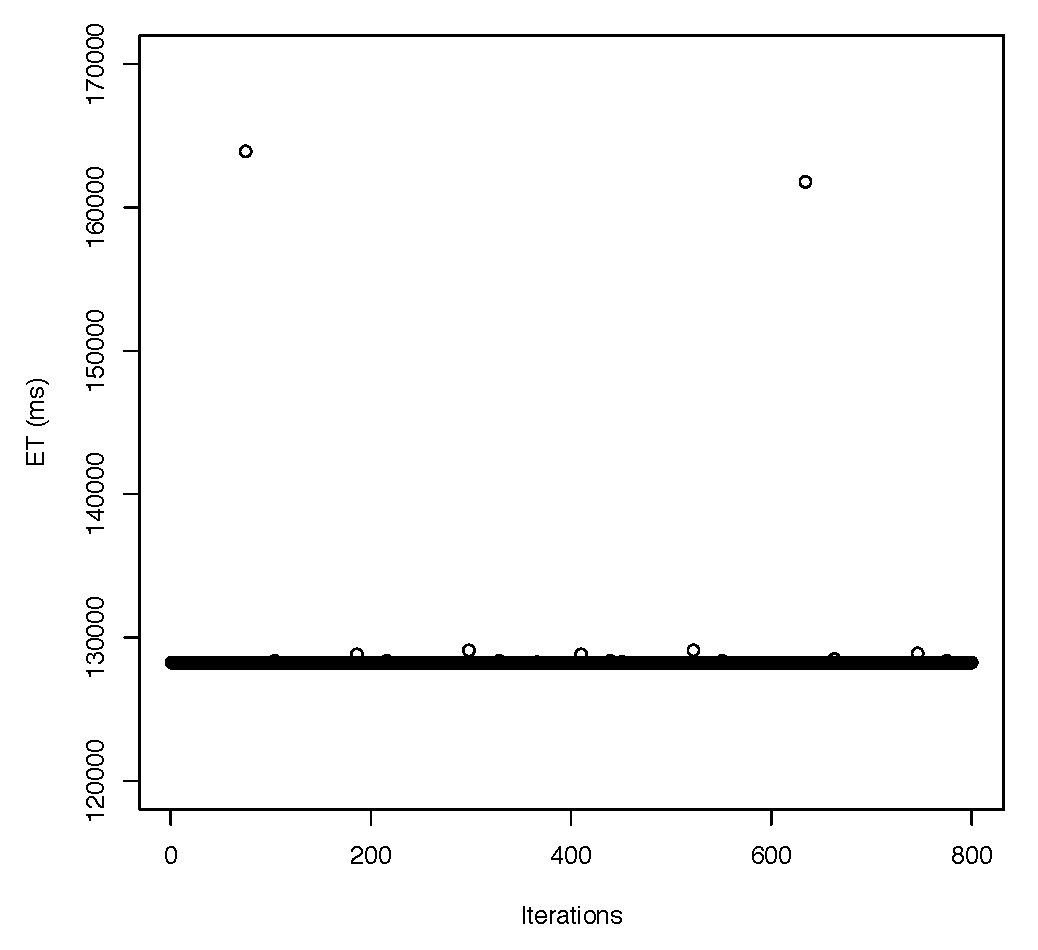
\includegraphics[width=0.223\textwidth]{put128_empv4_new.eps}
		\label{fig:reg_put128}
	}
	\subfigure[Dual-PUT256 Measurements]{
		%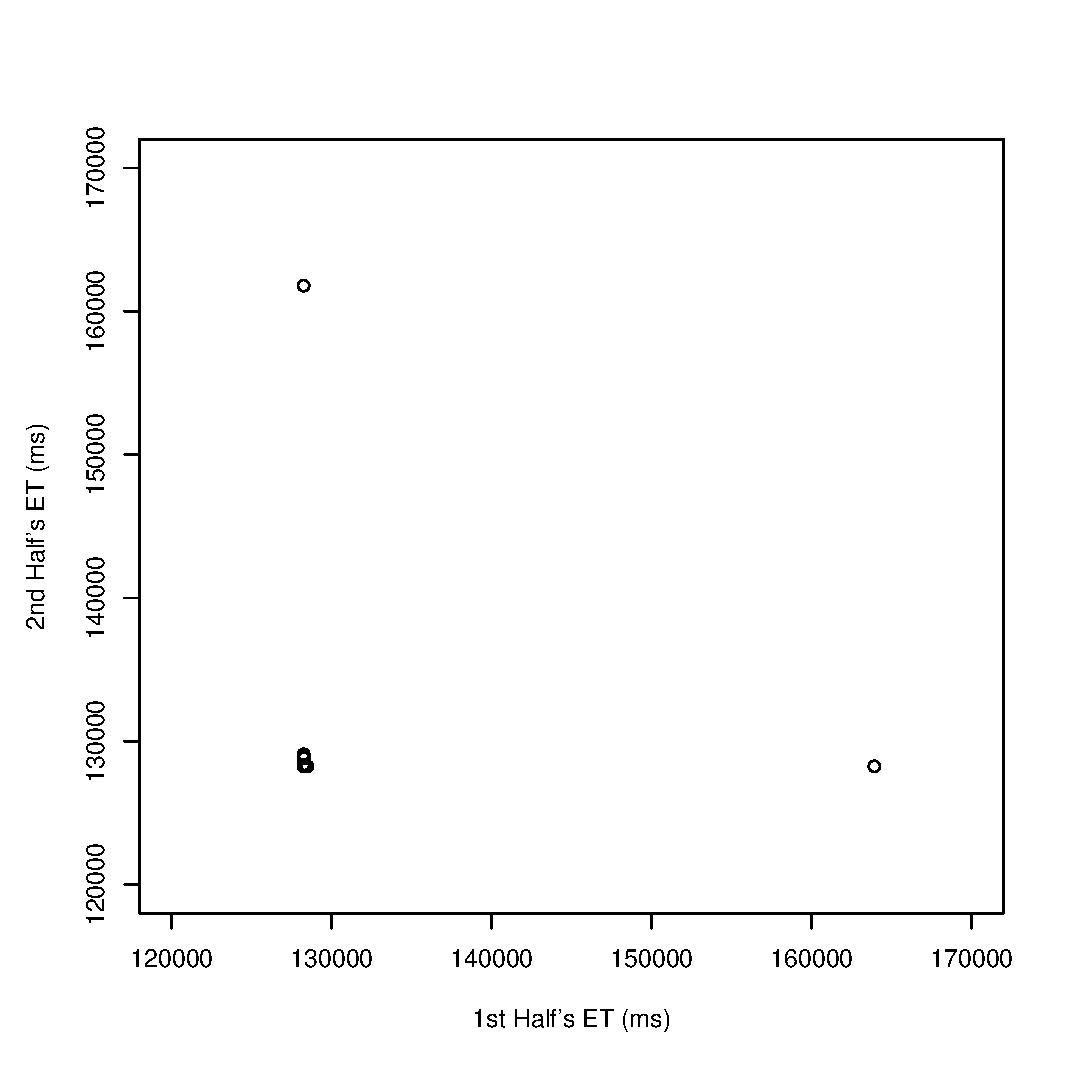
\includegraphics[width=0.223\textwidth]{dual_et_put256_empv4.eps}
		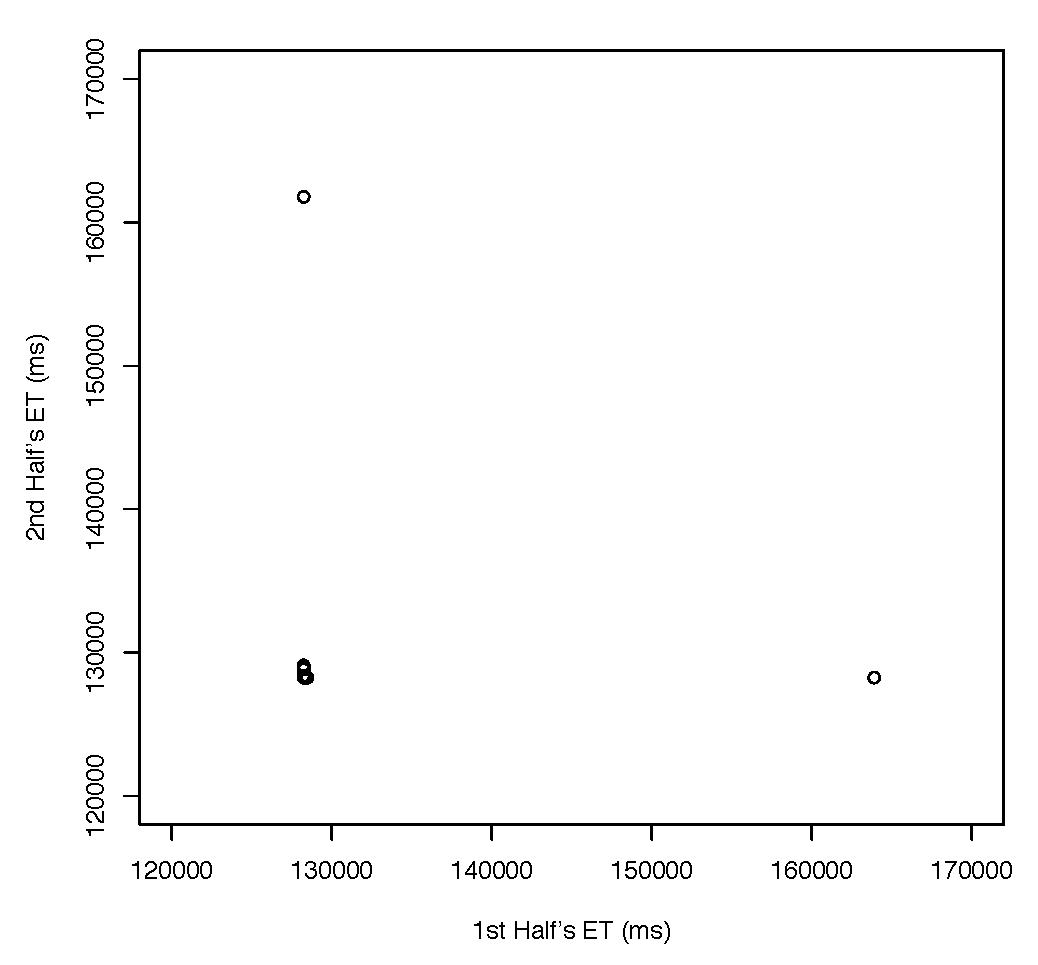
\includegraphics[width=0.223\textwidth]{dual_et_put256_empv4_new.eps}
		\label{fig:raw_put128}
	}
	%\vspace{-0.1in}    
	\subfigure[Zooming in on the $L$-shape]{
		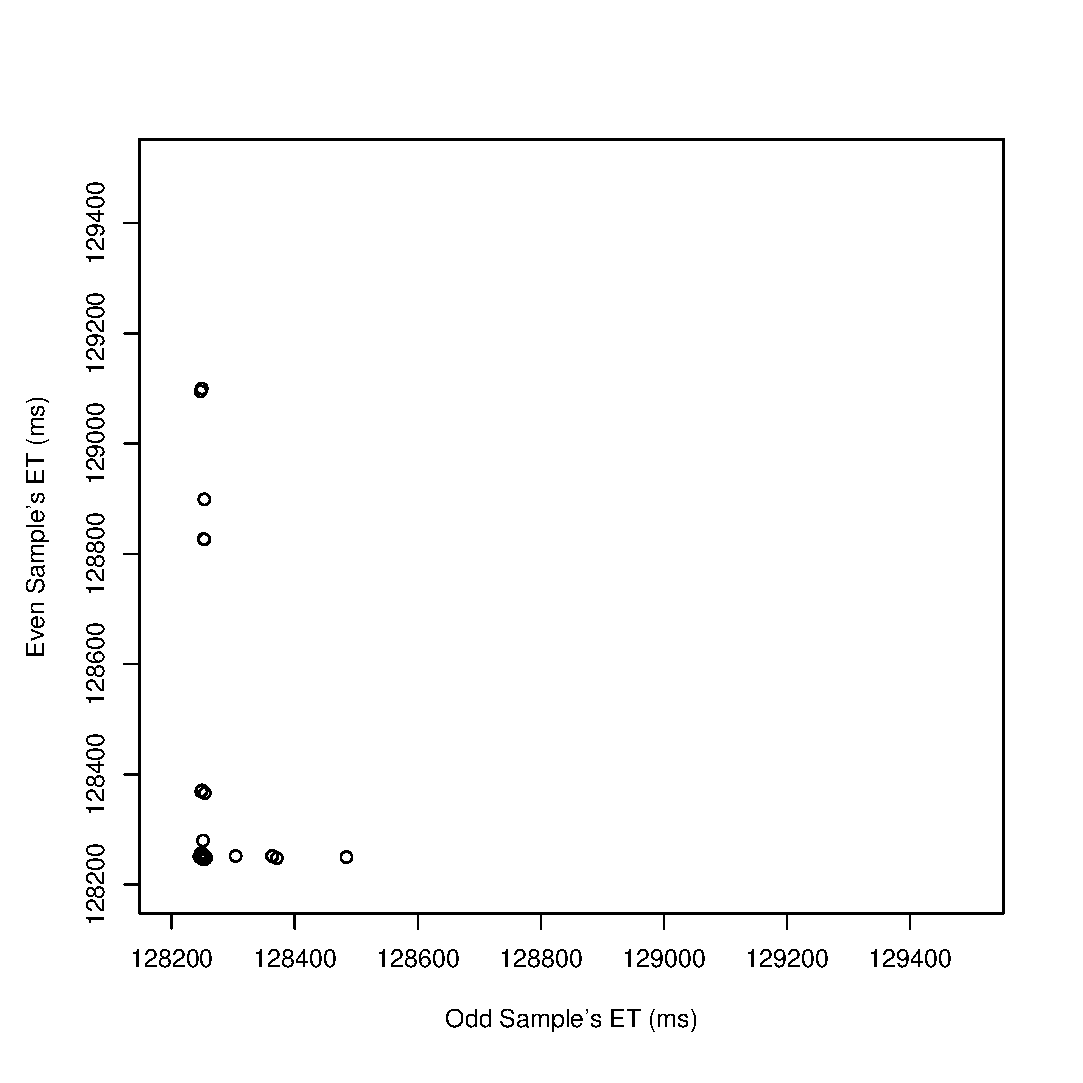
\includegraphics[width=0.223\textwidth]{zooming_in_dual_et_put256_empv4.eps}
		\label{fig:dual_put256_liters}
	}
%	\subfigure[Further Zooming in on the $L$-Shape]{
%		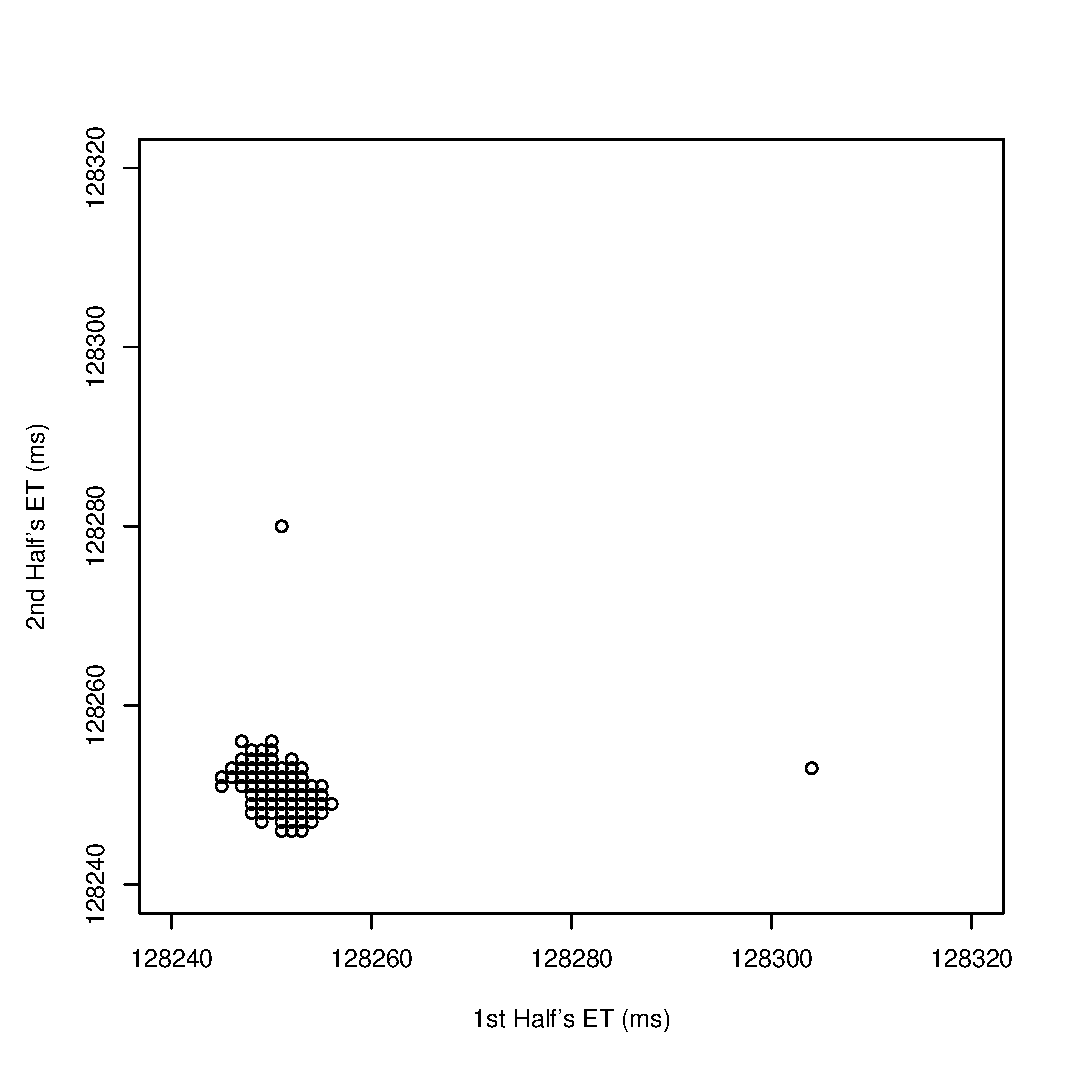
\includegraphics[scale=0.39]{further_zooming_in_dual_et_put256_empv4.eps}
%		\label{fig:fzoom_in_dual_et_put256}
%	}
	\subfigure[The Central Cluster]{
		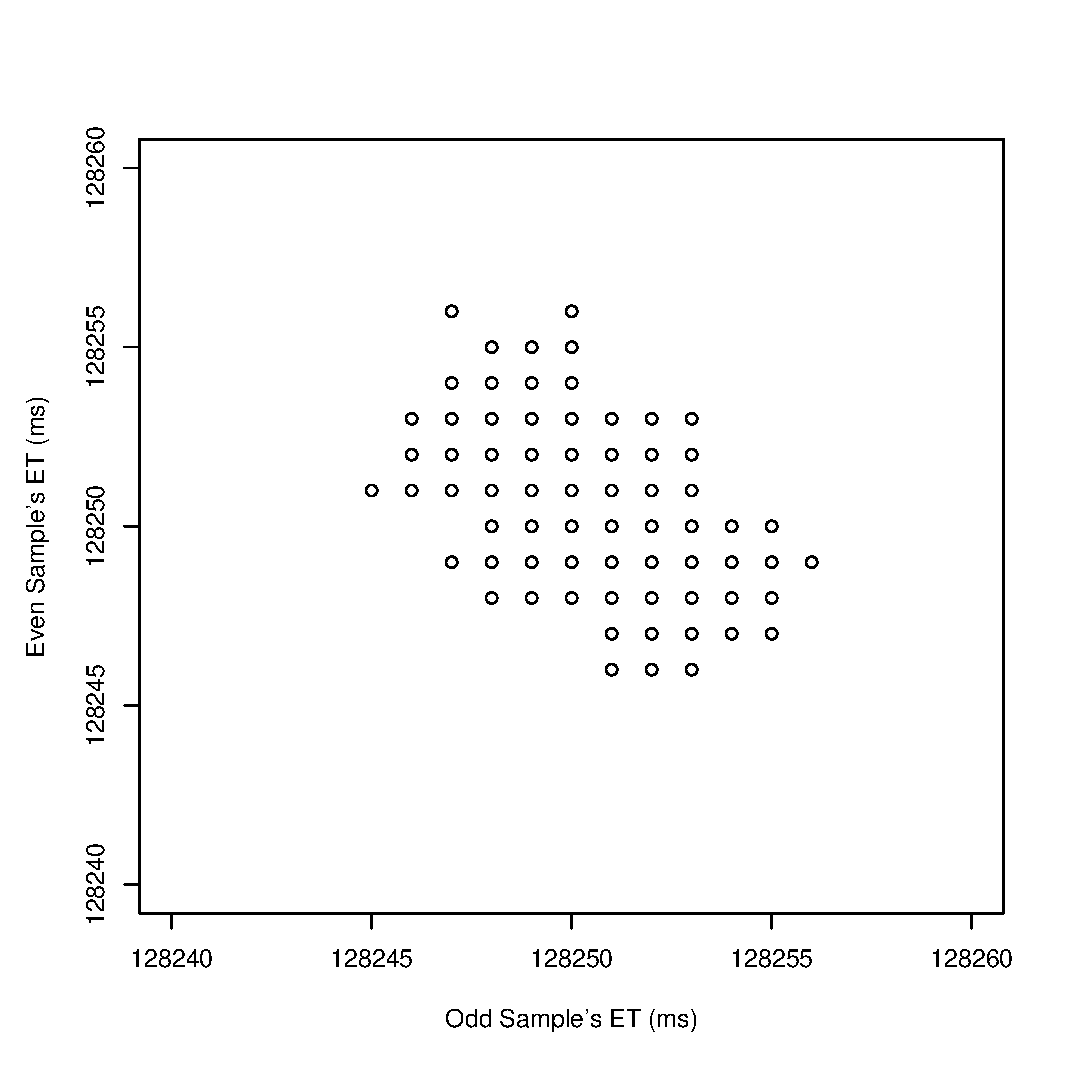
\includegraphics[width=0.223\textwidth]{dual_et_clump_put256_empv4.eps}
		\label{fig:dual_et_put256_cluster}
        }
    \caption{Successive Scatter plots of a PUT128 with 800 samples 
    (equivalent to a Dual-PUT256 with 400 samples) in Steps~2---4~\label{fig:put128_plot}} 
    \vspace{-0.3in}     
\end{figure} 

We informally term this phenomenon of a scatter plot of a dual-PUT run an
``$L$-shape,'' and attribute it to the
presence of infrequent long-running daemons.\shorten{Again, samples containing such
daemons (termed the $L$-samples) will appear
along the left y-axis or along the bottom x-axis, but will not occur in the
top right of the scatter plot of the dual-PUT.}

Figure~\ref{fig:dual_put256_liters} zooms into the lower left region,
focusing on the
tight cluster of samples.  Interestingly, this plot continues to exhibit an
$L$-shape, with perhaps a dozen or more $L$-samples in the left and bottom arms of
the ``$L$,'' and again no samples in the upper right portion of the
scatter plot.

We continue zooming until we get to Figure~\ref{fig:dual_et_put256_cluster},
which shows a central cluster (Step 4). 
We confirm the symmetry of the ET measurements in the central cluster: there
is no $L$-shape, and thus no $L$-samples, and thus no obvious infrequent
long-running daemons.\shorten{(We emphasize that these samples may have lots of
frequent daemons, as well as infrequent, {\em short-running} daemons.) There
were 384 dual-PUT256 samples in this central cluster, implying that 16 of
the PUT128 samples were $L$-samples and the 785 remaining of the original 800 PUT128
samples had no infrequent, long-running daemons, which motivates that term.}

We then perform Step~5, which computes 
the maximum process time and standard deviation 
of PT (process time, note the switch in emphasis from elapsed time 
to process time) of the daemon processes 
(e.g. {\tt cifsd}, {\tt flush-9:0}, {\tt jbd2/md0-8}, 
{\tt kblockd/0}, {\tt khugepaged}, {\tt md0\_raid1}, and {\tt ntpd})
observed in the central cluster samples in Fig.~\ref{fig:dual_et_put256_cluster}. 
\shorten{In the running example the maximum PT of those daemons was under 4 msec, 
and their standard deviation was just about 1 msec.}

In Step~6 we identify, for each daemon in the \hbox{$L$-samples}, 
those that are actual long-running daemon
executions.  We define such executions as those whose PT 
is over two standard deviations above the maximum PT for
that daemon in the central cluster samples. 
In the running example  {\tt flush-9:0}, 
{\tt jbd2/md0-8}, and {\tt md0\_raid1} 
are determined as infrequent, long-running.
We also identify ``extra'' infrequent daemons: those
found only in the $L$-samples but not in the central cluster. 
The running example reveals the following extra daemons: 
{\tt bash}, {\tt grep}, {\tt rhn\_check}, {\tt rhnsd}, {\tt rhsmcertd}, 
{\tt rhsmcertd-worke}, and {\tt sshd}.

For each of the infrequent daemons 
we use a heuristic to determine the daemon's periodicity: 
the daemon must occur regularly in a sequence of samples.
For instance, the {\tt rhn\_check} daemon appears 
roughly every 112 samples (which corresponds to very close to every four 
hours). Four others ({\tt flush-9:0}, {\tt jbd2/md0-8}, 
{\tt md0\_raid1}, and {\tt rhn\_check}) all occur together 
(in those two outliers in Fig.~\ref{fig:raw_put128}) and 
  have a periodicity of about every 559 samples
  (5x longer, or just about 20 hours). 
%  It is important only which samples a given daemon shows up 
%  in; we don't care in this heuristic whether daemons are co-occurring.

Next, we can compute for each so-identified infrequent, long-running daemon its
minimum time in the \hbox{$L$-samples} (Step 7). 
This computation provides a rough, initial distinction of a ``long-running''
daemon, namely, the valley between the maximum PT from the central cluster 
and the minimum PT from the $L$-samples, to differentiate ``short-running'' 
from ``\hbox{long-running}'' executions of the daemon. 
For those daemons (i.e. {\tt grep}) never appearing in the central cluster,
this initial analysis concludes only that they are infrequent.

In Step 8 we repeat Steps 1--6, but instead with the much-longer running
PUT16384 (4.5 hours per sample versus 2 minutes), to see 
if any of our identified infrequent daemons are actually frequent 
at that much longer PUT execution time. 
We find some frequent daemon processes appearing in both of the 
clusters of the dual-PUT256 and dual-PUT32768: 
{\tt flush-9.0}, {\tt jbd2/md0-8}, {\tt kblock/0}, {\tt md0\_raid1}, 
and {\tt ntpd}. That said, the central cluster also contains other
  processes not seen in the dual-PUT256 central cluster: 
  {\tt grep}, {\tt rhn\_check}, {\tt rhnsd}, {\tt rhsmcertd}, 
  {\tt rhsmcertd-worke}, and {\tt sshd}. 
  But these daemons were categorized in the \hbox{dual-PUT256} analysis as {\em
  infrequent}, several having periodicities estimated at four or twenty hours.
When the PUT had a ``short'' 
program time (in this case, two minutes), daemons with a periodicity of
hours are infrequent. But with a PUT with a ``long'' program time (in this
case, 4.5 hours), some of those daemons are now frequent, and appear in the 
central cluster.

In Step~9 we compute 
the cutoff for each of those infrequent, long-running daemons so
identified, based on the PUT128 and the 
PUT16384 as collected in Tab.~\ref{tab:final_infrequent_cutoff}. 
Here is how to compute the cutoff. For the cutoff of such a daemon with PUT128, 
we take the midpoint between the maximum of that daemon's PTs in the 
central cluster (or 0, if absent) and the minimum of those in the $L$-samples. 
For the cutoff of such a daemon with PUT16384, we do the same. 
We then compute a ``task time'' as 5\% of the inferred periodicity. 
This 5\% ensures that such infrequent daemons will impact 
only a small percentage of the shorter PUTs, while presumably being 
associated with much larger cutoffs for the very long PUTs. 
We also include daemons that (a)~were identified as infrequent and 
\hbox{long-running} from PUT128 and (b)~were not identified as so in the PUT16384 
\hbox{$L$-samples}, but may have in the \hbox{dual-PUT32768} central cluster. 
We then take the {\em maximum} of the two cutoffs for the final cutoff PT 
(the last column of Tab.~\ref{tab:final_infrequent_cutoff}). 

\begin{table}[h]
\centering
{\scriptsize
\begin{tabular}{|p{1.2cm}|c|c|p{1cm}|p{1.45cm}|} \hline
Process  & Cutoff PT & Cutoff PT & Task  & {\bf Final } \\
 Name & on PUT128  & on PUT16K & Time & {\bf Cutoff PT} \\\hline
{\tt bash} & 1 msec & --- & --- & {\bf 1 msec} \\ \hline
{\tt flush-9:0} & 64 msec & --- & $< 1$ hour & {\bf 64 msec} \\
                & ---     & 48 msec & $\geq 1$ hour & {\bf 48 msec} \\ \hline
{\tt grep }     & 1 msec & 12 msec & --- & {\bf 12 msec}\\ \hline
{\tt jbd2/md0-8} & 4 msec & --- & $< 1$ hour & {\bf 4 msec} \\
                & ---     & 11 msec & $\geq 1$ hour & {\bf 11 msec} \\ \hline
{\tt md0\_raid1} & 35 msec & ---     & $< 1$ hour  & {\bf 35 msec}\\
                 & ---     & 51 msec & $\geq 1$ hour & {\bf 51 msec} \\ \hline
{\tt rhn\_check}  & 281 msec & --- & $< 12$ min & {\bf 281 msec} \\
                 &  --- & 12,828 msec & $\geq 12$ min & {\bf 12,828 msec}\\ \hline
{\tt rhnsd} & 2 msec & --- & $< 12$ min & {\bf 2 msec} \\
            & ---    & 12 msec &$\geq 12$ min & {\bf 12 msec} \\ \hline
{\tt rhsmcertd}  & 1 msec & 1 msec & --- & {\bf 1 msec} \\  \hline
{\tt rhsmcertd}  & 57 msec & --- & $< 12$ min & {\bf 57 msec} \\
{\tt -worke}           &  --- & 119 msec  & $\geq 12$ min & {\bf 119 msec}\\ \hline
{\tt sshd} & 2 msec & 23 msec & --- & {\bf 23 msec}\\ \hline
\end{tabular}
}
\caption{Collected Infrequent, Long-running Daemons and Their Final Cutoff
  Process Time \hbox{(Step~9)}\label{tab:final_infrequent_cutoff}}
  \vspace{-0.4in}
\end{table}

Based on Tab.~\ref{tab:final_infrequent_cutoff}, 
we discard any sample containing an infrequent, long-running daemon execution
over the corresponding cutoff. We thus end up dropping just fifteen of the 800
PUT128 samples and only two of the forty PUT16384 samples. 
As a result, the overall measurement quality---the standard deviation and relative error 
---for PUT128 was improved 
by three orders of magnitude (as shown in Fig.~\ref{fig:meas_comp}) 
and by about two orders of magnitude for PUT16384.
%(5661.7 vs. 229.8) 0.0003448491 vs. 8.4$\times$10$^{-6}$
%(40.4 vs. 26.7) 2.463122e-06 vs. 1.626005e-06

%\begin{table}[H]
%\centering
%{\small
%\begin{tabular}{|c|c|c|} \hline
% & \multirow{2}{*}{ET/PT} & Std. Dev. & \multirow{2}{*}{Rel. Err.} \\ 
% & & &  & (msec) &  \\ \hline
%\multirow{2}{*}{PUT128} & ET & 800 & 2.5  & 2.0$\times$10$^{-5}$\\  \cline{2-9}
%  & PT & 2.6  & 2.0$\times$10$^{-5}$\\ \hline  
%\multirow{2}{*}{PUT16384} & ET & 138.6  & 8.4$\times$10$^{-6}$\\  \cline{2-9}
% & PT & 2.7  & 1.6$\times$10$^{-6}$\\ \hline  
%\end{tabular}
%}
%\caption{Measurement Statistics of PUT128 (above) and PUT16384 (below) 
%by the SEDONA Scheme\label{tab:refined_stat}}
%\end{table}

%We additionally remove those samples 
%in which the PT measurements are greater or less 
%two standard deviations from the average of the combined samples. In this
%particular case, no additional samples were removed.

%Finally, we calculate the execution time of PUT128 as the average PT measurement in Table~\ref{tab:refined_empv5}: 
%128250 milliseconds (rounded up to the nearest millisecond, because PT is
%measured in msec). Table~\ref{tab:refined_empv5} shows the statistics of 
%the PT and ET measurements. (In the fourth column, the number of samples
%dropped by the first sanity check (15 for ET) and by the second sanity check
%(1) are indicated.) Our original goal was to
%determine using a carefully-motivated protocol the program time (PT) for
%this program under test (PUT). We see that the standard deviation and
%relative error have both been considerably reduced by this principled
%elimination of samples containing identified infrequent, long-running daemons.

%\begin{table}[H]
%\centering
%{\small
%\begin{tabular}{|c|c|c|c|c|c|c|c|c|c|} \hline
% & \multirow{2}{*}{ET/PT} & \multirow{2}{*}{\# of Samples} & \multirow{2}{*}{\# of Ols. (=I+II)} & Min. & Max. & Avg. & Std. Dev. & \multirow{2}{*}{Rel. Err.} \\ 
% & & &  & (msec) & (msec) & (msec) & (msec) &  \\ \hline
%\multirow{2}{*}{PUT128} & ET & 800 & 16 (=15+1) & 128,245  & 128,256  & 128,250  & 2.5  & 2.0$\times$10$^{-5}$\\  \cline{2-9}
%  & PT & 800 & 20 (=15+5) & 128,245  & 128,255  & 128,250  & 2.6  & 2.0$\times$10$^{-5}$\\ \hline  
%\multirow{2}{*}{PUT16384} & ET & 40 & 6 (=2+4) & 16,416,454  & 16,417,155  & 16,416,637  & 138.6  & 8.4$\times$10$^{-6}$\\  \cline{2-9}
% & PT & 40 & 2 (=2+0) & 16,415,757  & 16,415,855  & 16,415,804  & 2.7  & 1.6$\times$10$^{-6}$\\ \hline  
%\end{tabular}
%}
%\caption{Statistics of PUT128 (above) and PUT16384 (below) by EMPv5\label{tab:refined_empv5}}
%\end{table}

\section{Evaluation}
\label{sec:eval}
\vspace{-0.07in}
We now evaluate the \hbox{performance} of the SEDONA protocol.
Our experiments were conducted on a machine
described in Table~\ref{tab:machine_config}. 
\begin{table}[h]
\vspace{-0.2in}
\begin{center}
{\scriptsize
\begin{tabular}{|l|p{7cm}|}\hline
OS & Red Hat Ent. Linux (RHEL) 6.4 with a kernel of 2.6.32 \\ \hline
CPU & Intel Core i7-870 Lynnfield 2.93GHz quad-core \hbox{processor}\shorten{ on a LGA 1156 95W motherboard}\\ \hline
RAM & 4GB of DDR3 1333 dual-channel memory\\ \hline
HDD & Western Digital Caviar Black 1TB 7200rpm SATA Drive\\ \hline
\end{tabular}
}
\end{center}
\caption{Machine Configurations\label{tab:machine_config}}
\vspace{-0.3in}
\end{table}

We evaluated the performance of the SEDONA using SPEC CPU2006 
benchmarks~\cite{specCpu2006}, providing various compute-bound real applications. 
%Thus, employing the SPEC benchmarks as real-world workloads 
%was a reasonable choice for the evaluation. 
The results are provided in Table~\ref{tab:spec_real}.
Note that in the table there are two empty bins associated with 
the {\tt 481} and {\tt 483} benchmarks. 
In the case of {\tt 481}, it was not possible to obtain its 
measurements of {\tt 481} due to some unknown error 
(perhaps caused by provided binary input data). 
As {\tt 483} concerned I/O, we excluded that benchmark. 
%Other than these two, we had successful runs of a total of 29 (out of 31) benchmarks. 

Table~\ref{tab:spec_real} shows that
the SEDONA protocol (which uses PT) significantly outperformed the original 
measurement technique (using ET), termed ORG, 
on the standard deviation and relative error across the different SPEC benchmarks. 
None of the benchmarks revealed a bigger standard deviation from the SEDONA
protocol as compared to that of ORG.
%All of the benchmarks revealed a smaller standard deviation on our scheme than that of the ORG. 
Our protocol quite effectively filtered out infrequent daemon executions 
in these real-world workloads. 
Furthermore, the relative error of SEDONA was equal to or 
lower than that of ORG for slightly under an half (specifically, 12) of the benchmarks.
%For instance, we observed about a 10x margin between the two schemes for the 
%{\tt 434} workload.

SEDONA also scaled well for the SPEC workloads, 
with regard to growth of relative error as the execution time lengthened.
For the short benchmarks 
(e.g., {\tt 400}, {\tt 403}, {\tt 410}, 
{\tt 434}, {\tt 445}, and {\tt 999}: those taking under 100 sec), 
our scheme outperformed the ORG by about 3.5x, on average. 
The SEDONA continued its dominance against the conventional technique 
for the medium-length benchmarks (e.g., {\tt 447}, {\tt 456}, {\tt 470}, and {\tt 473}).
For the long-running benchmarks (e.g., {\tt 436} and {\tt 454}, both$>$ 900 sec), 
the relative error of the \hbox{SEDONA} was slightly lower than that of the ORG.

%Lastly, we still observed a substantial standard deviation (and relative error) for 
%some benchmarks (e.g., {\tt 436} and {\tt 462}).
%The high variance seemed mainly attributed to the activities
%of the {\tt kslowd000} and {\tt kslowd001} daemon processes, as also identified in the real-world programs. 
%These two were not observed during our cutoff study. 
%The daemons cannot be switched off, as they involve kernel threads. 
%More investigation is needed to hopefully better remove 
%daemon executions interfering with timing a program.

%In summary, these results empirically demonstrate that measurement quality---accuracy,
%precision, and scalability---of EMP is also realized with real CPU-bound benchmarks.

\vspace{-0.1in}
\begin{table}[h]
\centering
{\scriptsize
\begin{tabular}{l|cc|cc} \hline
\multirow{2}{*}{Benchmarks} 
  & \multicolumn{2}{c|}{Std. Dev. (msec)} 
  & \multicolumn{2}{c}{Relative Error}\\ \cline{2-5}
  & {ORG} & {SEDONA} & {ORG} & {SEDONA}\\ \hline		
{{\tt 400.perlbench}} & {3} 	& {2} & {6$\times$10$^{-3}$} & {3$\times$10$^{-3}$}\\
{{\tt 401.bzip2}} & {1,185} & {1,161} & {2$\times$10$^{-3}$} & {2$\times$10$^{-3}$}\\
{{\tt 403.gcc}} & {138} & {96} & {5$\times$10$^{-3}$} & {4$\times$10$^{-3}$}\\
{{\tt 410.bwaves}} & {46} & {19} & {6$\times$10$^{-3}$} & {2$\times$10$^{-3}$}\\
{{\tt 416.gamess}} & {965} & {876} & {1$\times$10$^{-3}$} & {9$\times$10$^{-4}$}\\%% V
{{\tt 429.mcf}} & {623} & {600} & {3$\times$10$^{-3}$} & {3$\times$10$^{-3}$}\\
{{\tt 433.milc}} & {743} & {725} & {2$\times$10$^{-3}$} & {2$\times$10$^{-3}$}\\ %% V
{{\tt 434.zeusmp}} & {75} & {7} & {5$\times$10$^{-3}$} & {5$\times$10$^{-4}$}\\
{{\tt 435.gromacs}} & {947} & {900} & {1$\times$10$^{-3}$} & {9$\times$10$^{-4}$}\\
{{\tt 436.cactusADM}} & {3,914} & {3,843} & {3.37$\times$10$^{-3}$} & {3.36$\times$10$^{-3}$}\\
{{\tt 437.leslie3d}} & {1,492} & {1,475}  & {3$\times$10$^{-3}$} & {3$\times$10$^{-3}$}\\
{{\tt 444.namd}} & {294} & {281}  & {5$\times$10$^{-4}$} & {5$\times$10$^{-4}$}\\
{{\tt 445.gobmk}} & {91} & {28}  & {1$\times$10$^{-3}$} & {3$\times$10$^{-4}$}\\
{{\tt 447.dealII}} & {150} & {108}  & {3$\times$10$^{-4}$} & {2$\times$10$^{-4}$}\\
{{\tt 450.soplex}} & {99} & {91}  & {3$\times$10$^{-4}$} & {2$\times$10$^{-4}$}\\
{{\tt 453.povray}} & {623} & {582}  & {2$\times$10$^{-3}$} & {2$\times$10$^{-3}$}\\
{{\tt 454.calculix}} & {678} & {627}  & {3.9$\times$10$^{-4}$} & {3.7$\times$10$^{-4}$}\\
{{\tt 456.hmmer}} & {85} & {50}  & {2$\times$10$^{-4}$} & {1$\times$10$^{-4}$}\\
{{\tt 458.sjeng}} & {542} & {513} &  {9$\times$10$^{-4}$} & {9$\times$10$^{-4}$}\\
{{\tt 459.GemsFDTD}} & {2,143} & {2,132}  & {3$\times$10$^{-3}$} & {3$\times$10$^{-3}$}\\
{{\tt 462.libquantum}} & {3,326} & {3,274}  & {6$\times$10$^{-3}$} & {6$\times$10$^{-3}$}\\
{{\tt 464.h264ref}} & {601} & {563}  & {9$\times$10$^{-4}$} & {9$\times$10$^{-4}$}\\
{{\tt 465.tonto}} & {883} & {797}  & {1$\times$10$^{-3}$} & {1$\times$10$^{-3}$}\\
{{\tt 470.lbm}} & {143} & {94} & {4$\times$10$^{-4}$} & {3$\times$10$^{-4}$}\\
{{\tt 471.omnetpp}} & {2,114} & {2,072} & {6$\times$10$^{-4}$} & {6$\times$10$^{-4}$}\\
{{\tt 473.astar}} & {359} & {317} &  {1$\times$10$^{-3}$} & {9$\times$10$^{-4}$}\\
{{\tt 481.wrf}} & \multicolumn{4}{c}{Run-time Error}\\
{{\tt 482.sphinx3}} & {2,436} & {2,392} &   {4$\times$10$^{-3}$} & {4$\times$10$^{-3}$}\\ %% V
{{\tt 483.xalancbmk}} & \multicolumn{4}{c}{Out-of-Scope}\\
{{\tt 998.specrand}} & {0.6} & {0.6} &  {4$\times$10$^{-3}$} & {4$\times$10$^{-3}$}\\
{{\tt 999.specrand}} & {0.8} & {0.6} &  {6$\times$10$^{-3}$} & {5$\times$10$^{-3}$}\\ \hline
\end{tabular}
}
\caption{Performance Evaluation on the SPEC Benchmarks\label{tab:spec_real}}
\vspace{-0.33in}
\end{table}

%Figure~\ref{fig:real_performance} shows the evaluation results 
%of the proposed scheme on the running program-under-test with increasing task length in seconds.
%\begin{figure*}[t]
%	\centering
%	\subfigure[Standard Deviation]{
%		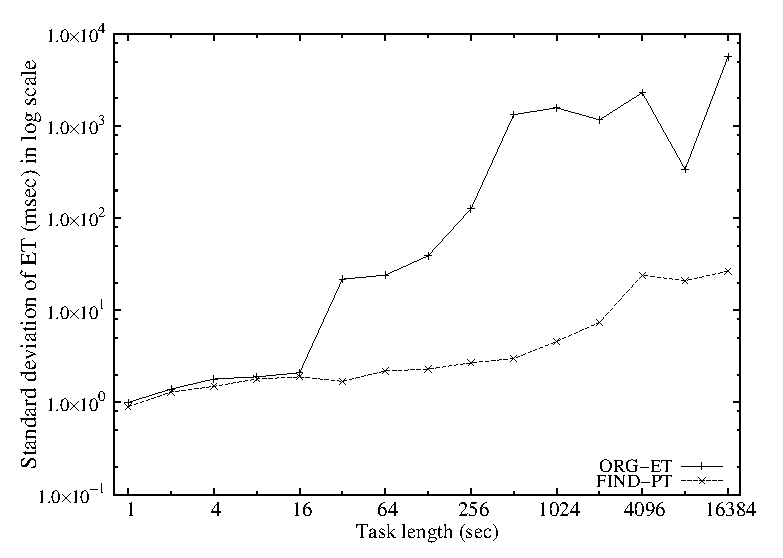
\includegraphics[width=0.45\textwidth]{all_put_std.eps}\label{fig:all_put_std}
%	} 
%	\subfigure[Relative Error]{
%		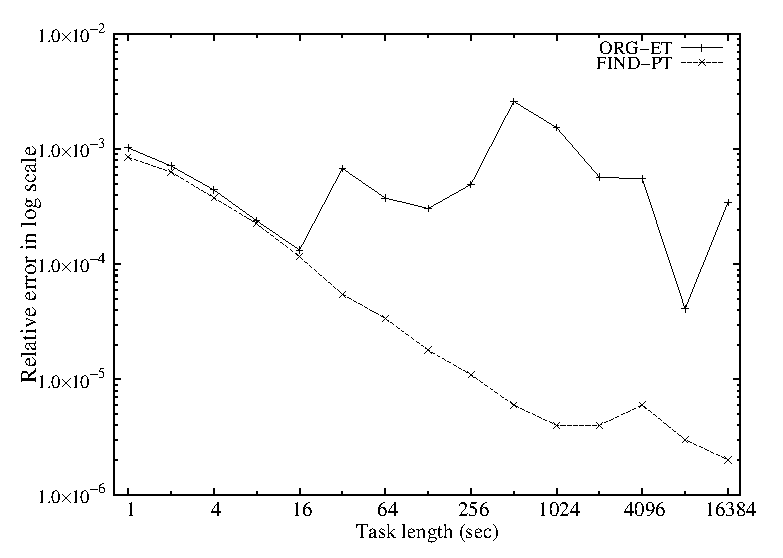
\includegraphics[width=0.45\textwidth]{all_put_re.eps}\label{fig:all_put_re}
%	}
%	\caption{Comparison of Measurement-Quality over Increasing Task Length~\label{fig:all_put}}
%\end{figure*} 

%Figure~\ref{fig:real_performance} shows the evaluation results 
%of the proposed scheme on an industrial benchmark, called SPEC CPU2006~\cite{specCpu2006}.
%\begin{figure*}[t!]
%	\centering
%	\subfigure[Standard Deviations]{
%		%\resizebox{width=.8\textwidth}{!}{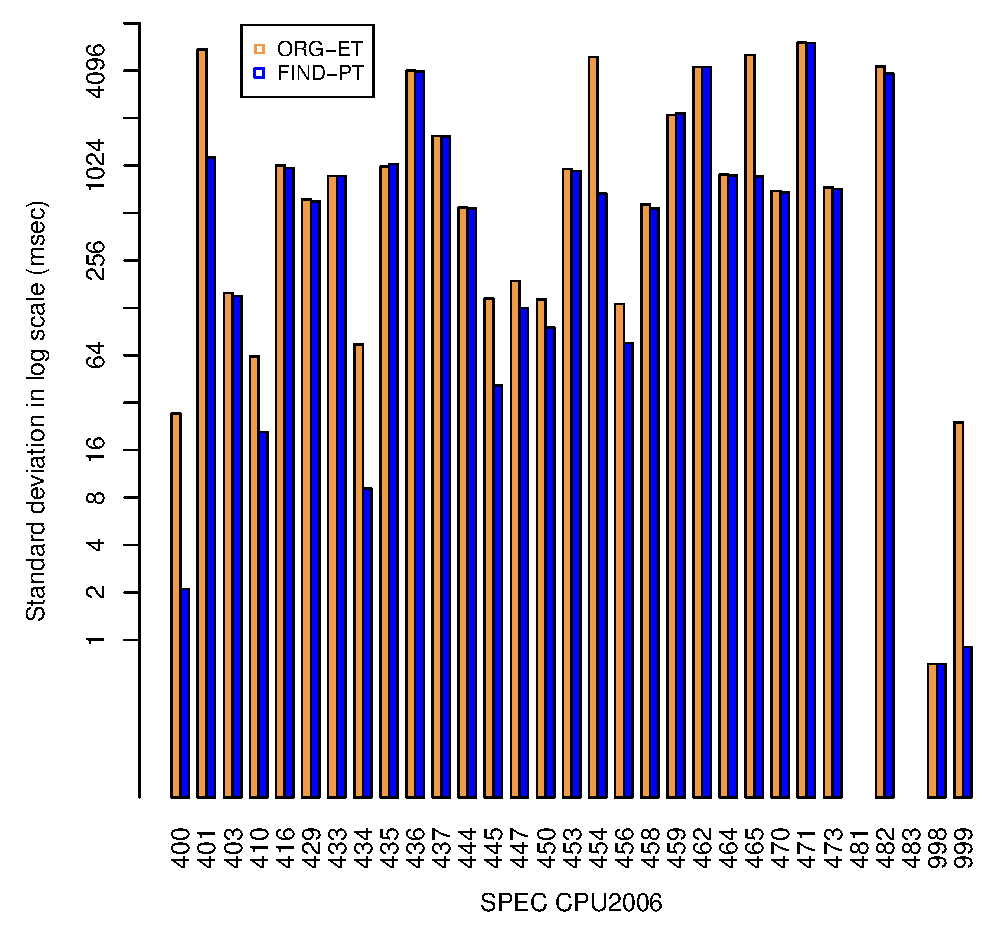
\includegraphics[width=140mm,height=]{spec_std.eps}\label{fig:spec_std}}
%		%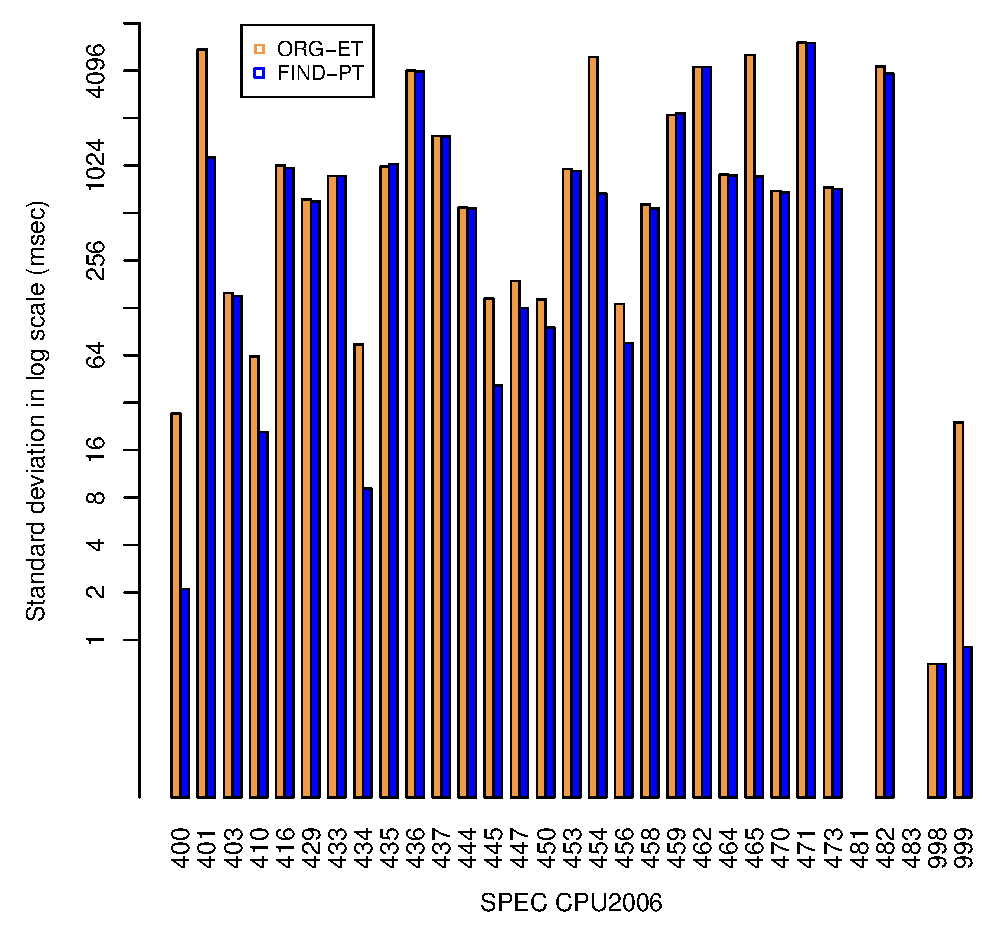
\includegraphics[width=\textwidth,height=3in]{spec_std.eps}\label{fig:spec_std}
%		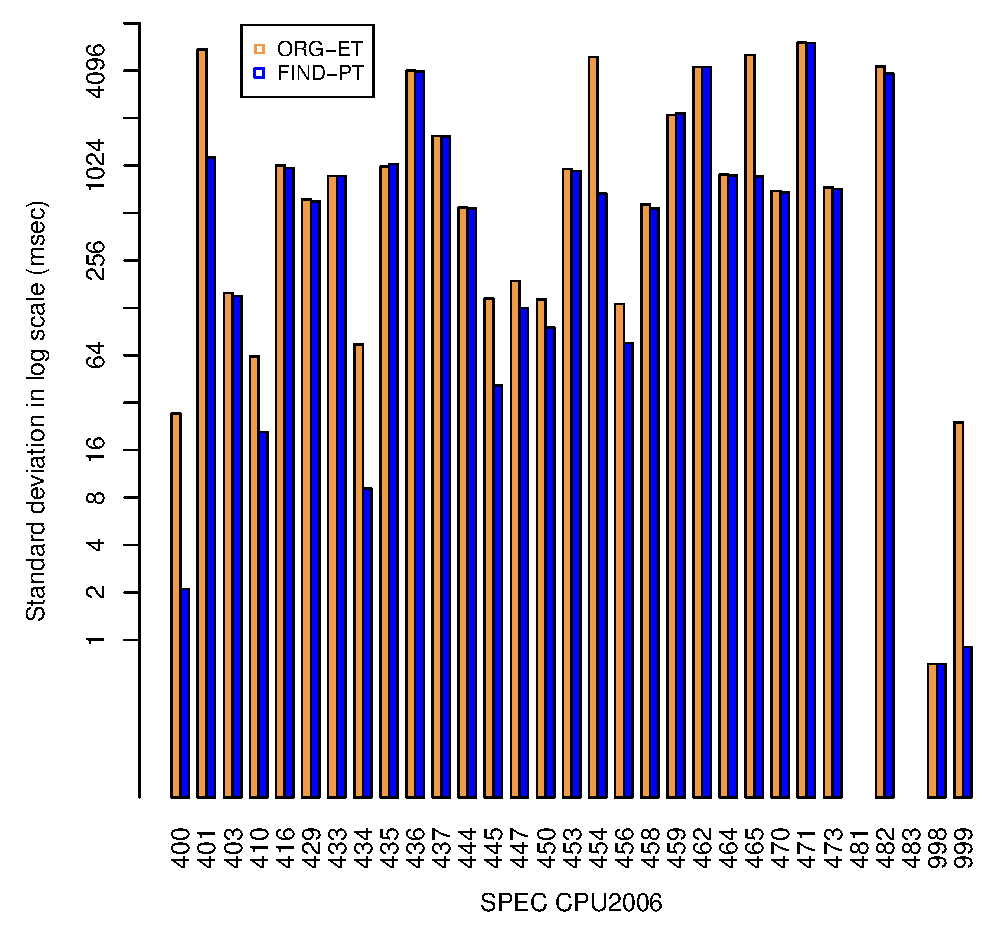
\includegraphics[scale=0.5]{spec_std.eps}\label{fig:spec_std}
%	} 
%	\subfigure[Relative Errors]{
%		%\vspace{-1in}
%		%\resizebox{.8\textwidth}{!}{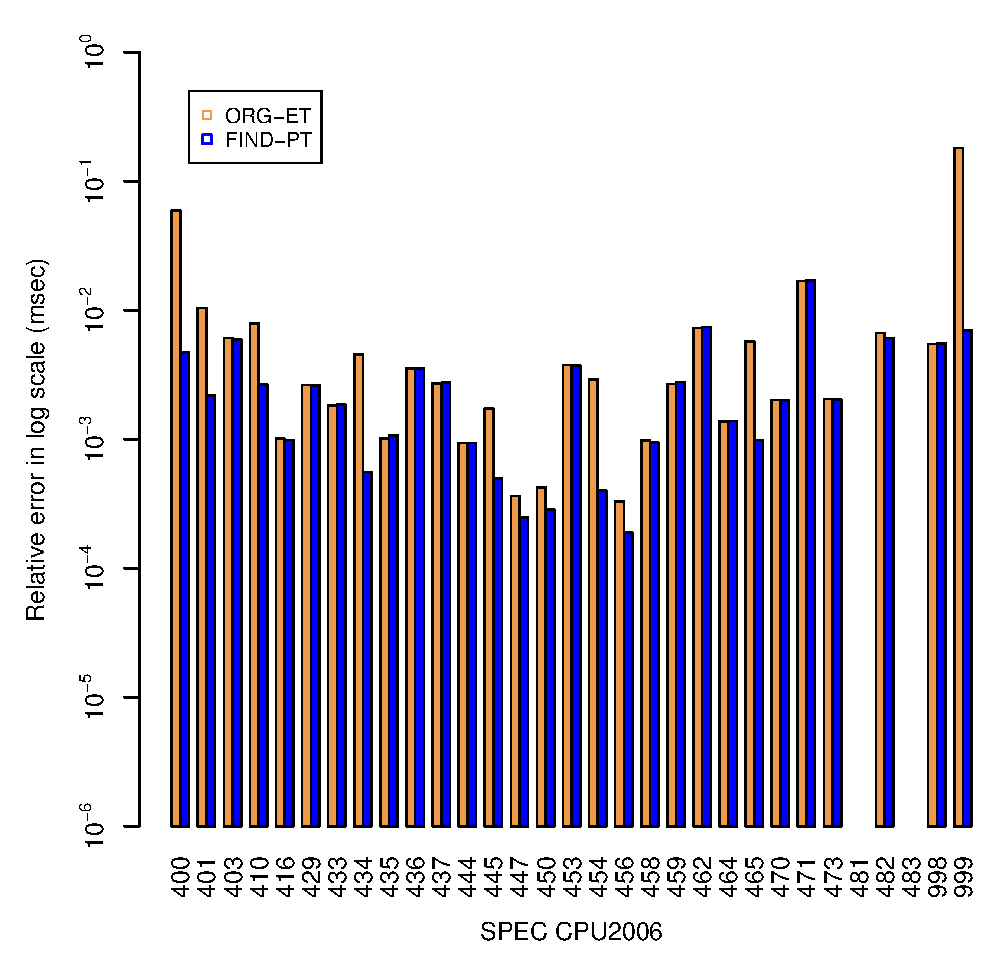
\includegraphics[width=140mm]{spec_re.eps}\label{fig:spec_std}}
%		%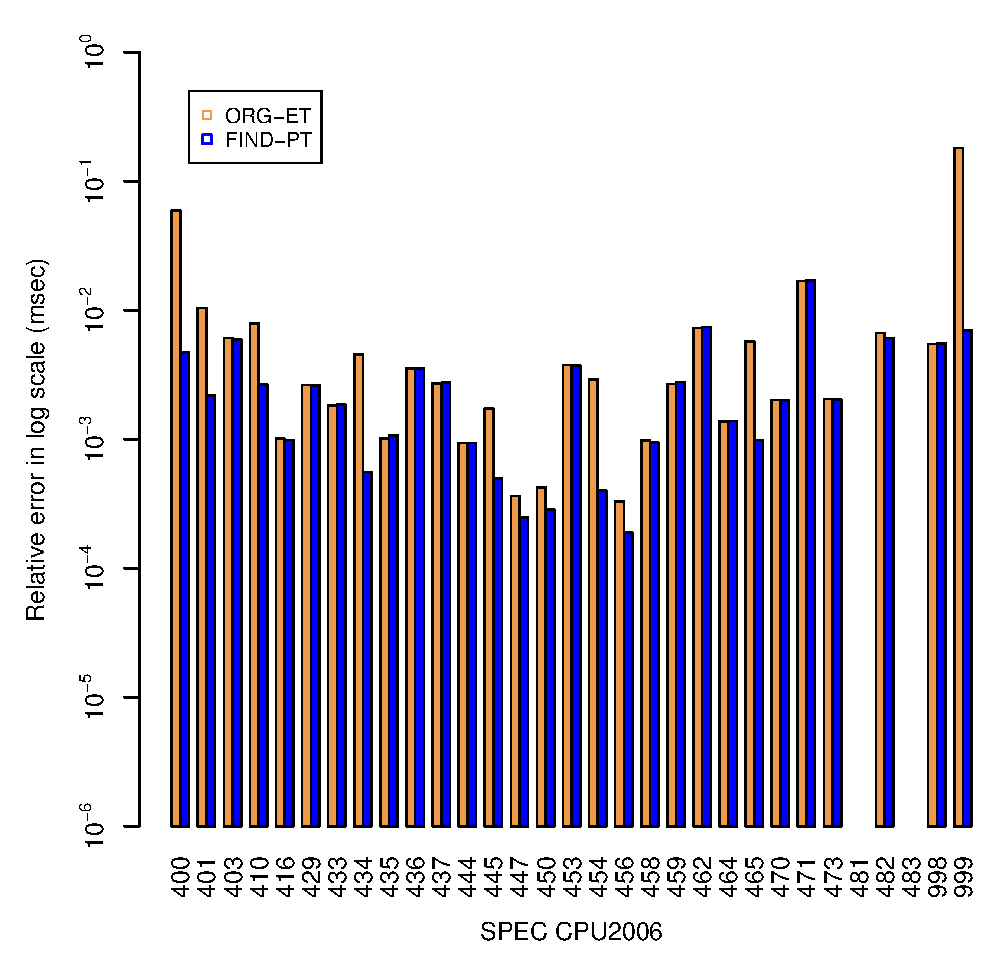
\includegraphics[width=\textwidth,height=3in]{spec_re.eps}\label{fig:spec_re}
%		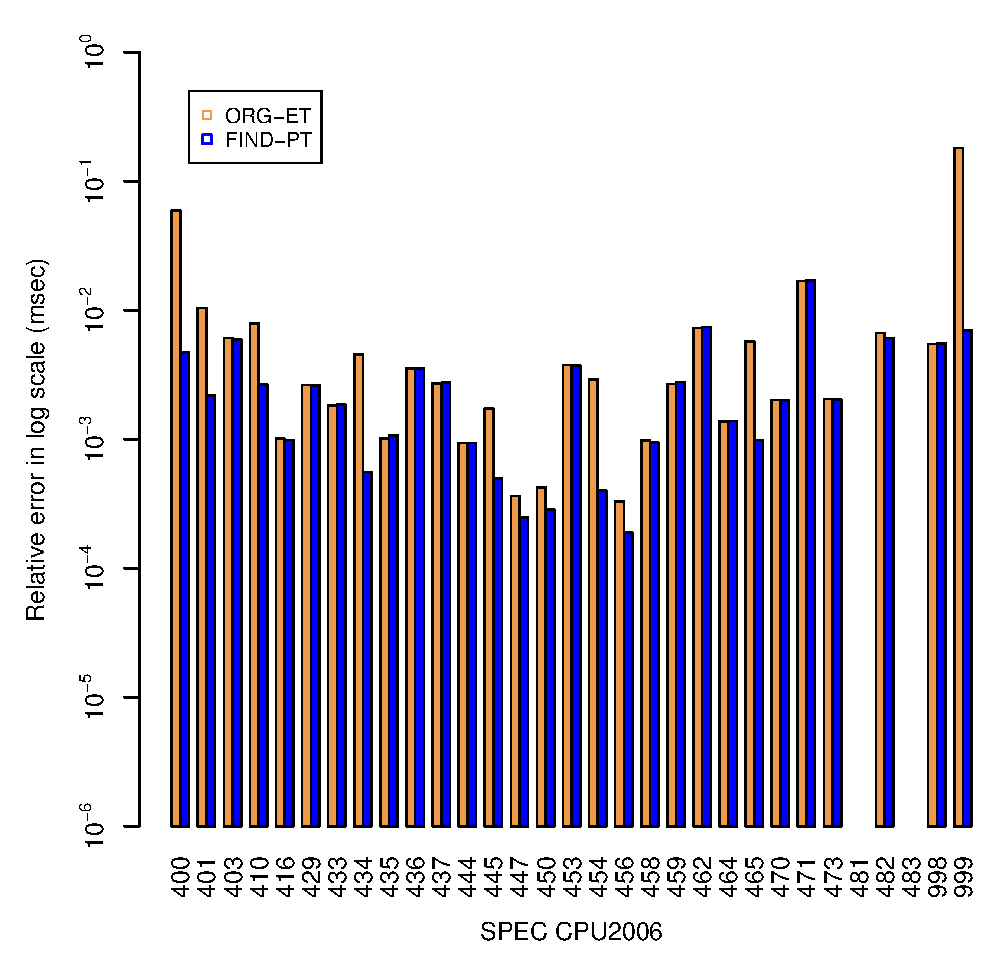
\includegraphics[scale=0.5]{spec_re.eps}\label{fig:spec_re}
%		%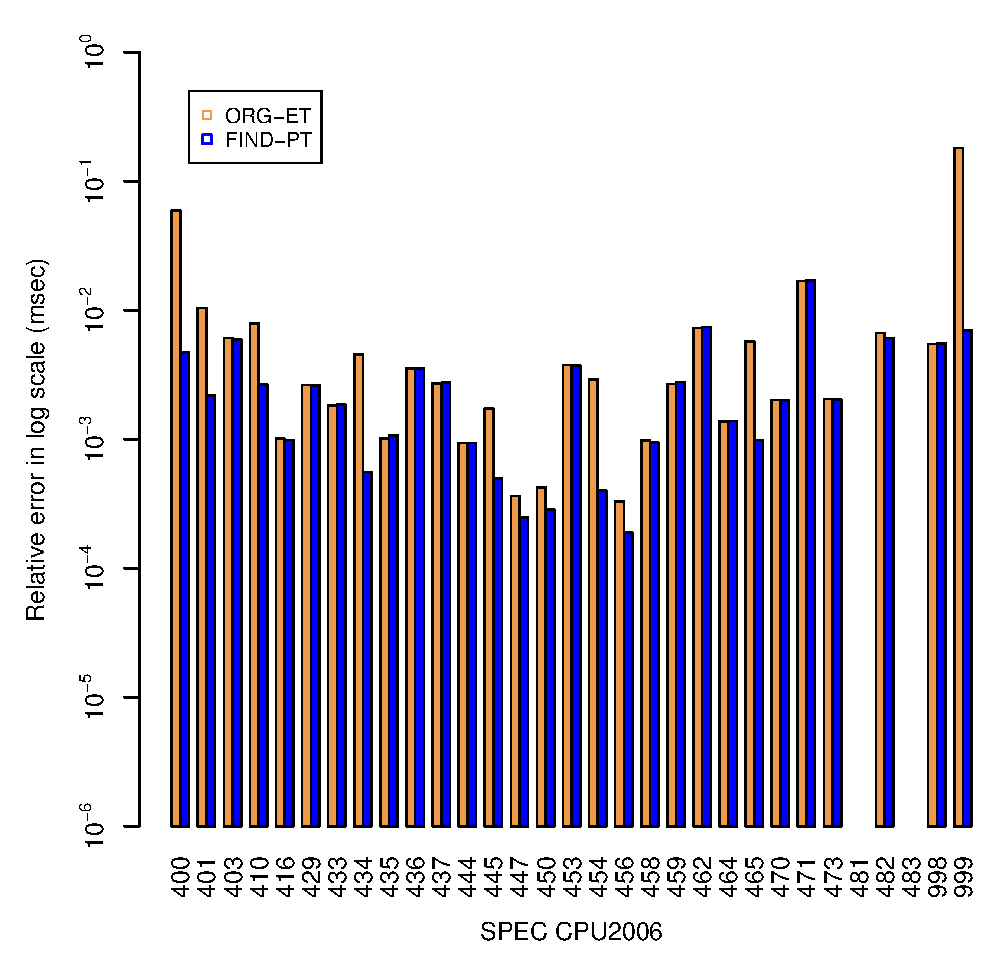
\includegraphics[scale=0.5]{spec_re.eps}\label{fig:spec_re}
%	}
%	\caption{Timing Performance over SPEC CPU2006~\label{fig:real_performance}}
%\end{figure*} 

\section{Conclusion}
\label{sec:conclusion}
\vspace{-0.07in}
In this paper we \shorten{provided an empirical evidence of 
how significantly measurement quality could be hurt by 
the presence of infrequent, long-running daemon processes. 
We }presented a novel execution-time measurement scheme called {\em SEDONA}\shorten{, 
employing process time and identifying an infrequent, long-running daemon}. 
%Our evaluation using real benchmarks demonstrated the strong effectiveness of 
%the scheme in improving the measurement performance.
Our scheme is more precise and accurate than the traditional method\shorten{
as shown in the experiments}.

% In the future we plan to integrate this approach into a novel query timing 
% protocol~\cite{Currim} to further improve the protocol by 
% early identifying such a daemon and eliminating samples contaminated by that daemon.

%\section*{Acknowledgments} 
%The author give many thanks to Rick Snodgrass, Rob Meier, and John Kececioglu 
%for their exceptional supports and helpful comments to improve this paper.

{\tiny 
\bibliographystyle{ieicetr} 
\bibliography{paper}
}
\end{document}
